MongoDBは高性能でオープンソース、モードレスなドキュメント型データベースです。これはリレーショナルデータベースとノンリレーショナルデータベースの間のプロダクトです。ノンリレーショナルデータベースの中では機能が最も豊富で、リレーショナルベースに最もよく似ています。サポートされるデータ形式は非常にルーズで、jsonによく似たbjson形式によってデータを保存します。そのため、比較的複雑なデータを保存することができます。Mongoの最大の特徴は検索言語が非常に強力でその文法がオブジェクト指向の検索文に少し似ていることです。データベースに対してインデックスを設定することもできます。

下の図はmysqlとmongoDBの間の対応関係を示しています。非常に簡単だとわかりますが、mongoDBの性能は非常に良いです。

\begin{figure}[H]
  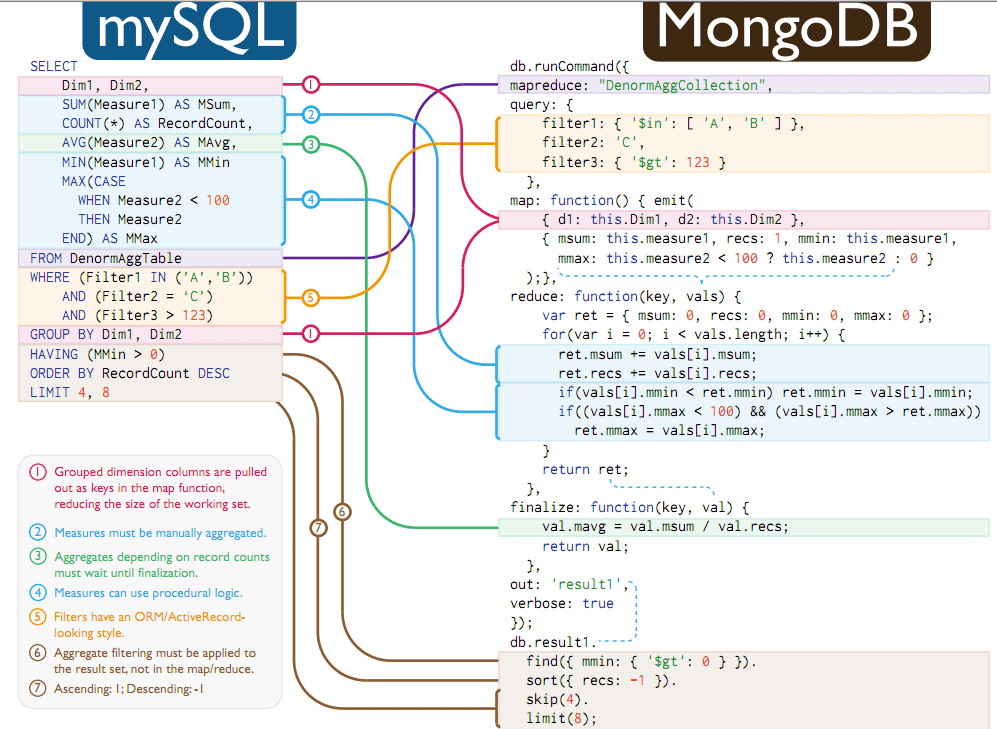
\includegraphics[width=14cm]{5.6.mongodb.png}
   \label{図5.1}
   \caption{MongoDBとMysqlの操作の対応図}
\end{figure}

現在GoでサポートされているmongoDBのもっとも良いドライバはmgo(http://labix.org/mgo)です。このドライバは現在もっともオフィシャルのpkgになりそうなものです。

次にどのようにしてGoからmongoDBを操作するのかご説明します:

\begin{lstlisting}[numbers=none]
package main

import (
    "fmt"
    "gopkg.in/mgo.v2"
    "gopkg.in/mgo.v2/bson"
    "log"
)

type Person struct {
    Name  string
    Phone string
}

func main() {
    session, err := mgo.Dial("server1.example.com,server2.example.com")
    if err != nil {
        panic(err)
    }
    defer session.Close()

    // Optional. Switch the session to a monotonic behavior.
    session.SetMode(mgo.Monotonic, true)

    c := session.DB("test").C("people")
    err = c.Insert(&Person{"Ale", "+55 53 8116 9639"},
        &Person{"Cla", "+55 53 8402 8510"})
    if err != nil {
        log.Fatal(err)
    }

    result := Person{}
    err = c.Find(bson.M{"name": "Ale"}).One(&result)
    if err != nil {
        log.Fatal(err)
    }

    fmt.Println("Phone:", result.Phone)
}
\end{lstlisting}

mgoの操作方法とbeedbの操作方法はほとんど似ていることがわかります。どちらもstructに基づいて操作する方法です。これこそがGo Styleです。
